%=====================================================================
\section{Results}
\label{sec:results}
The results follow the four parts of \cref{sec:methods}. Each subsection presents
the applicable datasets and their available evidence;
\cref{sec:r-cross} collects the verdicts. The CIT results below are measured outputs of all five B experiments, including
40 citation-target null graphs. Blue text elsewhere denotes untested expectations
for PS/CM, and grey boxes denote their pending figures. These draft expectations
are not evidence in the measured summary.
% One file per part; owners (PLAN.md section 5) are marked inside each file.
\subsection{Aggregation and time windows}
\label{sec:r-aggregation}

% Owner: A
\paragraph{Contact and messaging networks (PS, CM).}
\outline{Which conclusions are stable under window choice, and over which
$\Delta t$ range?}
\expect{[Expected] Density and clustering of the snapshots rise quickly with
$\Delta t$ and approach the aggregate only for windows comparable to the whole
observation period. The giant component of short-window snapshots is small, and
percolates at a window that is much shorter for CM than for PS because PS has a
daily rhythm (lessons, breaks). Conclusions about ``the'' clustering or density of
the network therefore depend strongly on $\Delta t$.}

\begin{figure*}[t]
\centering
\figph{0.32\textwidth}{3.6cm}{density vs.\ $\Delta t$\\(PS, CM)}\hfill
\figph{0.32\textwidth}{3.6cm}{clustering vs.\ $\Delta t$\\(PS, CM)}\hfill
\figph{0.32\textwidth}{3.6cm}{giant component vs.\ $\Delta t$\\(PS, CM)}
\caption{Structural metrics of snapshots as functions of the window length
$\Delta t$; dashed lines show the static aggregate. (Placeholder.)}
\label{fig:agg-window}
\end{figure*}

% Owner: B
% Owner: B -- measured CIT contribution only.
\paragraph{Citation network (CIT).}
In 2020, annual and cumulative graphs on the same 19,150 born nodes contain
1,450 and 73,269 citations. Mean total degree is 0.151 versus 7.652, weak
largest-component fraction 0.052 versus 0.641, and cumulative weak clustering
0.124. Annual clustering is identically zero: strict older-target citations make
each annual snapshot bipartite. This is a consequence of the representation,
not independent evidence for temporal correlations. Over 1-, 2-, 5- and 10-year
windows, relative ranges average 1.798 for density/degree, 2.361 for clustering
and 1.114 for largest-component fraction.
\textbf{CIT verdict on H1:} window choice changes structural descriptions;
some differences are definitional. The node denominator and year convention
must accompany every comparison.

\begin{figure*}[t]
\centering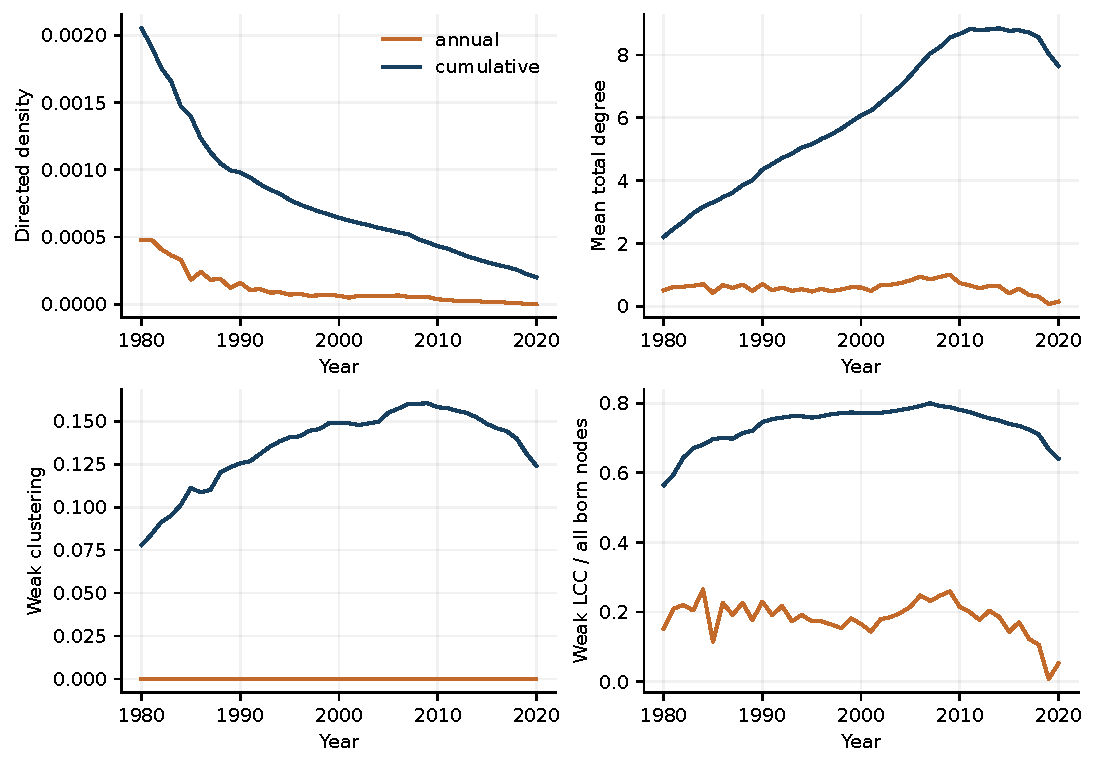
\includegraphics[width=.95\textwidth]{b_aggregation.pdf}
\caption{Measured CIT annual and cumulative structure, including born isolates.
The annual zero clustering is imposed by strict publication-year ordering.}
\label{fig:b-aggregation}
\end{figure*}

\paragraph{Window interpretation.}
\Cref{fig:b-window} shows that longer windows connect a larger fraction of born
papers and admit cross-year triangles. These effects require a sequence of
snapshots; one final aggregate cannot reveal when connectivity appears.
The relative range is a window-sensitivity statistic, not a significance test
against a temporal null, and identical density/degree sensitivity follows from
the common denominator.

\begin{figure*}[t]
\centering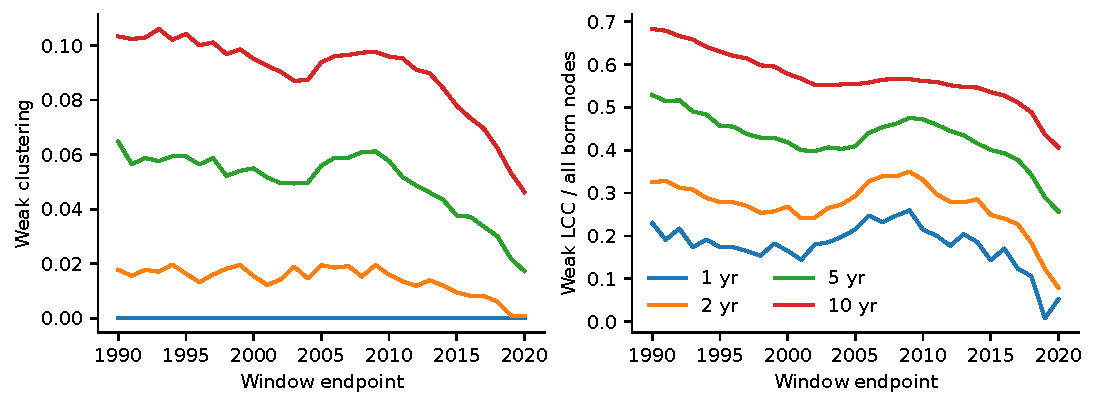
\includegraphics[width=.95\textwidth]{b_window_sensitivity.pdf}
\caption{Measured CIT trailing-window clustering and connectivity for 1, 2, 5
and 10 years. Born isolates are included at every endpoint.}
\label{fig:b-window}
\end{figure*}


\paragraph{Verdict on H1.}
Supported for CIT under the stated node denominator and strict-year convention.
A comparative verdict for PS and CM awaits their measurements; the relative
sensitivity of network types cannot yet be ranked.
 % Part I   (A, B)
\subsection{Activity patterns}
\label{sec:r-activity}

% Owner: C
\paragraph{Burstiness and memory.}
\expect{[Expected] Inter-event times of both PS and CM are heavy-tailed and have
positive burstiness $B$ and memory $M$. Under P1 the heavy tail is largely
removed, so $B_{\mathrm{real}}-B_{\mathrm{null}}>0$. Contact bursts in PS are
bounded by the school timetable, while CM shows longer waiting times (hours to
days) and a stronger tail.}

\begin{figure}[t]
\centering
\figph{\columnwidth}{3.6cm}{inter-event time distributions, real vs.\ P1\\(PS, CM)}
\caption{Inter-event time distributions on log--log axes. (Placeholder.)}
\label{fig:iet}
\end{figure}

\begin{table}[t]
\centering
\small
\begin{tabular}{@{}lcccc@{}}
\toprule
 & \multicolumn{2}{c}{PS} & \multicolumn{2}{c}{CM} \\
 & real & P1 & real & P1 \\
\midrule
Burstiness $B$ & $>0$ & $\approx$ lower & $>0$ & $\approx$ lower \\
Memory $M$ & $>0$ & $\approx 0$ & $>0$ & $\approx 0$ \\
\bottomrule
\end{tabular}
\caption{Expected qualitative outcome of M2a (values to be measured; mean $\pm$
std over $\geq 20$ P1 samples).}
\label{tab:burst}
\end{table}

% Owner: C
\paragraph{Persistence and turnover.}
\expect{[Expected] Many contacts in PS are repeated within the same day (within
class), so the edge repetition rate is high and consecutive-snapshot Jaccard is
moderate, with drops at class changes. In CM most pairs interact only a few
times, so tie lifetimes are short and turnover is high. P1 keeps the static graph
and therefore the repetition rate, but changes lifetimes and Jaccard.}

\paragraph{Verdict on H2 and H3.}
\outline{Supported / not supported / depends on network type or window.}
\expect{[Expected] H2 supported in both. H3 supported in PS, only partly in CM.}
    % Part II  (C)
\subsection{Structural evolution}
\label{sec:r-evolution}

% Owner: B
% Owner: B -- measured M2c-1 through M2c-4 only.
\paragraph{Preferential attachment (H4a).}
The conditional kernel $(k+1)^\alpha$ gives $\alpha=0.714$, with a descriptive
95\% year-bootstrap interval $[0.693,0.730]$. Twenty P3a samples yield
$0.0006\pm0.0051$ and age-only P3b yields $-0.6512\pm0.0053$.
The observed exponent exceeds all null values (empirical one-sided probability
$1/21$ per comparison, with coarse resolution). The exponent stays positive
under time splits, offsets 0.5/2 and a core venue-family subset.
\textbf{Verdict:} sublinear degree preference is supported within this corpus,
beyond the age-only reference; this does not identify a causal PA mechanism.

\paragraph{Ageing (H4b).}
Lognormal target preference is preferred to exponential, power-law and uniform
kernels, with respective $\Delta$AIC 537.8, 9,360.5 and 41,796.7.
The lognormal parameters are $(\mu,\sigma)=(1.858,1.108)$; its underlying scale
$e^\mu$ is 6.41 years. Mean age over all retained citations is 5.711 years, versus
$11.457\pm0.034$ for P3a and $5.717\pm0.018$ for calibrated P3b.
Lognormal is preferred in all three target cohorts, although recent-cohort tails
remain censored. \textbf{Verdict:} age-independent choice is inadequate;
P3b's agreement is calibration, not independent confirmation of ageing.

\begin{figure*}[t]
\centering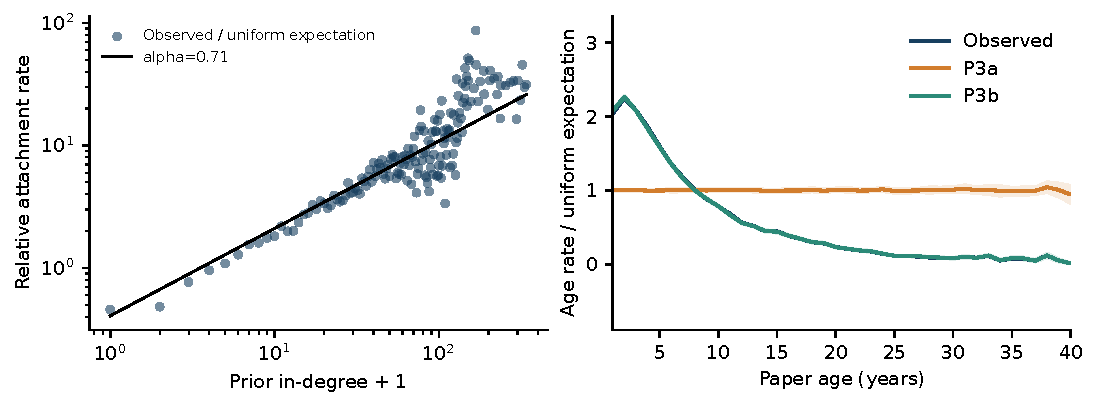
\includegraphics[width=.95\textwidth]{b_attachment_ageing.pdf}
\caption{Measured CIT attachment and exposure-adjusted age preference.
Points with at least five hits are displayed; the exponent uses all supported
classes with yearly normalization. Null bands show mean $\pm$ SD.}
\label{fig:growth}
\end{figure*}

\paragraph{Densification and diameter (H4c).}
For 1990--2020, $a=1.343$ ($R^2=0.991$), with descriptive year-resampling
interval $[1.288,1.406]$. Growth is weaker in 2005--2020 ($a=1.065$) than
1990--2004 (1.455); cutoff 2015 gives 1.427, inclusion of year ties 1.324,
and the core venue subset 1.410. Densification is superlinear edge growth,
not increasing directed density. The sampled weak-LCC effective diameter is
6 hops in every year; 64/256-source endpoint checks agree.
P3 fixes $N(t)$ and $E(t)$, hence also $a$.
\textbf{Verdict:} densification is observed, but diameter shrinkage is not
detected at the sampled 90th-percentile resolution.

\begin{figure*}[t]
\centering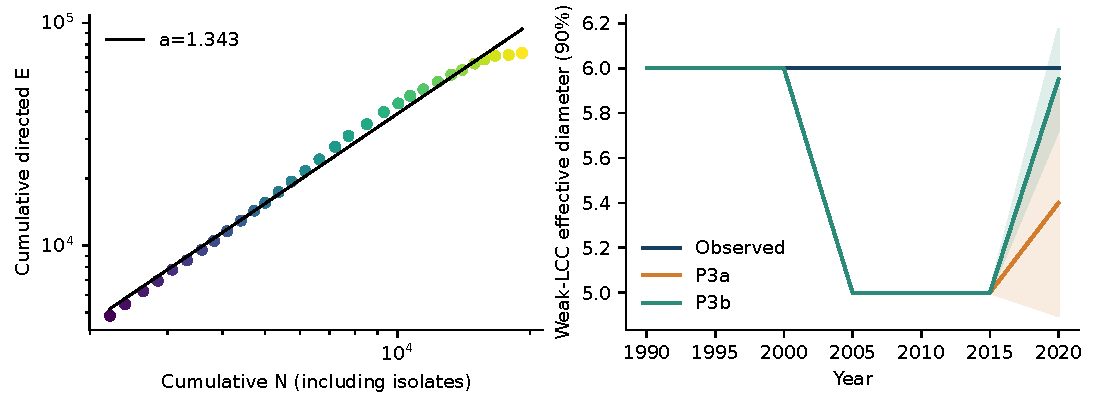
\includegraphics[width=.95\textwidth]{b_densification_diameter.pdf}
\caption{CIT cumulative growth and effective diameter. Null diameter means and
SD are estimated every five years. P3 cannot test densification significance
because its source reference counts are fixed.}
\label{fig:b-densification}
\end{figure*}

\paragraph{Citation dynamics and prediction (H4d).}
For 500 full-history fits, median WSB parameters are
$(\lambda,\mu,\sigma)=(2.717,0.834,1.238)$, median RMSLE is 0.074 and
scaled-collapse RMSE is 0.022. These are fitted-sample diagnostics.
On 500 papers selected using only their first five years, age-15 MAE is
15.144 for WSB, 17.064 for linear extrapolation and 27,588 for no-ageing PA;
at the observed 2020 endpoint it is 28.016, 27.271 and $2.79\times10^6$.
The paired MAE differences WSB minus linear have 95\% intervals
$[-4.471,0.806]$ and $[-4.764,8.128]$, both including zero. Forecast fits hit
parameter bounds for 38.6\% of papers; all remain in primary scoring.
\textbf{Verdict:} compact descriptive fits are supported, but a clear predictive
advantage over the simple linear baseline is not established. Observed-endpoint
citations are censored within-corpus counts, not lifetime impact.

\begin{figure*}[t]
\centering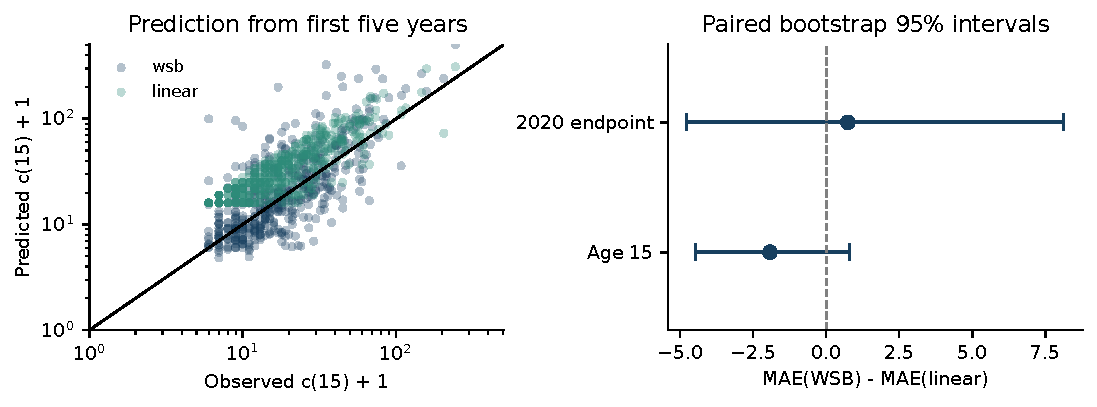
\includegraphics[width=.95\textwidth]{b_wsb_validation.pdf}
\caption{WSB held-out prediction and paired MAE differences versus linear.
Both bootstrap intervals cross zero; fitted collapse alone does not establish
long-term predictability.}
\label{fig:b-wsb-validation}
\end{figure*}


% Owner: E
\paragraph{Dynamic vs.\ static communities.}
\expect{[Expected] In PS the static partition recovers the classes well, but
snapshots reveal mixing during breaks and re-formation of classroom groups during
lessons, so consecutive NMI is moderate and fluctuates with the timetable. In CM
snapshot communities are unstable (low consecutive NMI), and P1 lowers
consecutive NMI further. Results should be insensitive to the resolution parameter
within a reasonable range.}

\begin{table}[t]
\centering
\small
\begin{tabular}{@{}lcc@{}}
\toprule
 & PS & CM \\
\midrule
Consecutive NMI & medium & low \\
Dynamic vs.\ static NMI & medium & low \\
NMI with classes & high (static) & -- \\
\bottomrule
\end{tabular}
\caption{Expected qualitative outcome of M4 (values and P1 baseline to be measured).}
\label{tab:nmi}
\end{table}

\paragraph{Verdict on H5.}
\outline{Supported / not supported / depends on network type or window.}
\expect{[Expected] H5 supported for CM, and in PS tied to
the daily timetable.}
   % Part III (B, E)
\subsection{Paths, centrality and spreading}
\label{sec:r-function}

% Owner: D
\paragraph{Reachability.}
\expect{[Expected] The fraction of pairs connected by a time-respecting path is
well below the static value in both networks. Under P1 reachability changes
because temporal order is destroyed, whereas P2 changes it through topology,
so the two nulls attribute the loss to different causes.}

\begin{figure}[t]
\centering
\figph{\columnwidth}{3.4cm}{reachability ratio $R$: real, P1, P2 (PS, CM)}
\caption{Temporal reachability ratio, real vs.\ P1 and P2. (Placeholder.)}
\label{fig:reach}
\end{figure}

% Owner: E
% Owner: E. M3b / H6 (rankings), input from results_function.tex.
% Values: results/e_summary.csv and results/e/m3b_*; figure: scripts/plot_e.py.
\begin{table}[t]
\centering
\small
\begin{tabular}{@{}llcc@{}}
\toprule
 & Measure & Real & P1 \\
\midrule
PS & $\tau$, unweighted & 0.71 & $0.55\pm0.01$ \\
   & $\tau$, weighted & 0.39 & $0.69\pm0.01$ \\
   & top-10\%, unweighted & 0.50 & $0.51\pm0.07$ \\
   & top-10\%, weighted & 0.29 & $0.60\pm0.06$ \\
\midrule
CM & $\tau$, unweighted & 0.78 & $0.85\pm0.00$ \\
   & $\tau$, weighted & 0.74 & $0.86\pm0.00$ \\
   & top-10\%, unweighted & 0.65 & $0.74\pm0.01$ \\
   & top-10\%, weighted & 0.57 & $0.72\pm0.02$ \\
\bottomrule
\end{tabular}
\caption{Agreement of static and temporal closeness rankings: Kendall $\tau_b$ and
overlap of the top 10\% nodes. P1: temporal closeness on 20 samples (mean $\pm$ sd); the
static ranking is unchanged by P1.}
\label{tab:m3b}
\end{table}

\begin{figure*}[t]
\centering
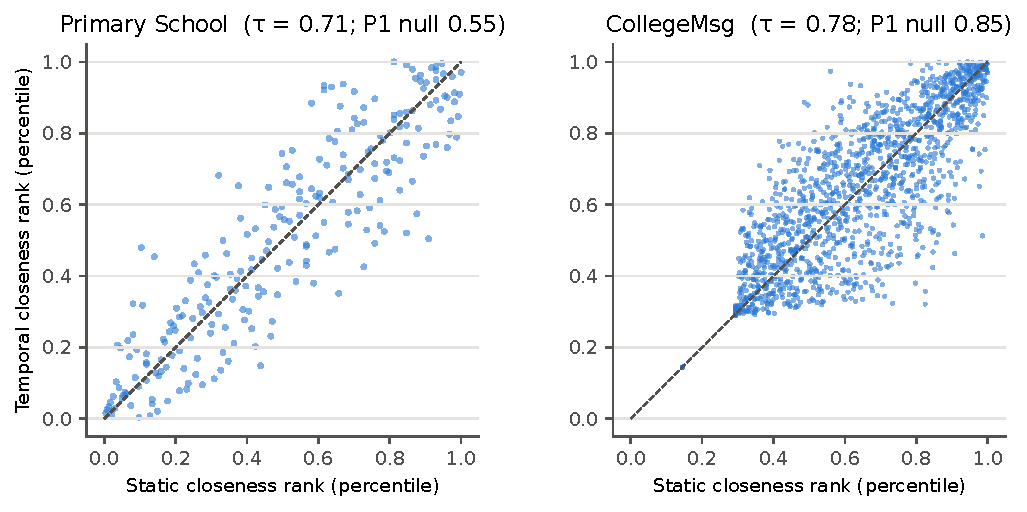
\includegraphics[width=0.8\linewidth]{e_m3b_rank_scatter.pdf}
\caption{Static (unweighted harmonic) vs.\ temporal closeness rank of every node; dashed:
identical rankings. The tied block at the lower left of the CM panel is the 29\% of users
who never send a message.}
\label{fig:m3b}
\end{figure*}

\paragraph{Centrality.}
Static and temporal closeness rankings are clearly correlated in both networks
(\cref{tab:m3b,fig:m3b}; $\tau=0.71$ in PS and $0.78$ in CM, hop distance), so the static
network shows roughly which nodes are central. It is much less reliable about which nodes
are \emph{most} central: only half of the PS top 10\% and two thirds of the CM top 10\%
coincide. In CM the real agreement is somewhat lower than under P1 (0.78 vs.\ 0.85), so
event order makes static closeness a slightly worse guide. The CM $\tau$ is also helped by
the 549 users (29\%) who never send a message and have zero closeness in both rankings
(the tied block in \cref{fig:m3b}).

In PS the effect depends on edge weights. Weighted static closeness agrees poorly with
temporal closeness ($\tau=0.39$, top-10\% overlap 0.29), whereas after P1 the agreement
is high ($0.69\pm0.01$). In the school, most contact weight comes from repeated contacts
within a class during lessons; these happen while the class is already connected and
hardly shorten time-respecting paths to the rest of the school. Under P1 the same contacts
are spread over the day, and a heavy edge becomes a frequent chance to transmit. Without
weights the effect reverses (real 0.71 vs.\ P1 0.55): reaching the school quickly depends
on having many distinct partners, which in PS largely means mixing at breaks.

\emph{Rankings part of H6: partly supported.} The rankings are correlated
($\tau=0.71$--$0.78$) but the top nodes differ by 35--50\%, and in face-to-face data
weighting edges by contact frequency makes the static ranking misleading ($\tau=0.39$).


% Owner: D
\paragraph{Spreading.}
\expect{[Expected] SIR epidemics on the real sequences peak later than on P1,
$T_{\mathrm{real}}/T_{\mathrm{null}}>1$, and the effect is larger for the
burstier CM. In PS, the final size is limited by the timetable (outbreaks pause
overnight).}

\begin{figure}[t]
\centering
\figph{\columnwidth}{3.4cm}{SIR prevalence curves: real, P1, P2 (PS, CM)}
\caption{Mean SIR prevalence with $\geq 100$ seeds. (Placeholder.)}
\label{fig:sir}
\end{figure}

\paragraph{Verdict on H6 and H7.}
\outline{Supported / not supported / depends on network type or window.}
\expect{[Expected] H6 supported in both networks. H7 supported, strongest for CM.}
    % Part IV  (D, E)
\subsection{CIT model diagnostics and robustness}
\label{sec:b-diagnostics}
% Owner: B. All diagnostics use the completed CIT run, not new experiments.
\paragraph{Null controls and ageing alternatives.}
\Cref{fig:b-null-age} visualizes the separation of the observed attachment
exponent from both null ensembles and the age-kernel AIC comparison.
P3b matches mean citation age because its age weights were fitted to these data;
that agreement is a property of the control, not independent evidence for ageing.
With only 20 realizations per null, an observed value above all nulls has empirical
one-sided probability $1/21$; this does not justify a precise tail estimate.
The ageing comparison is on identical risk sets and observations.

\begin{table}[t]
\centering\small
\begin{tabular}{@{}lrr@{}}
\toprule
Age kernel & Parameters & $\Delta$AIC\\
\midrule
Lognormal & 2 & 0.0\\
Exponential & 1 & 537.8\\
Power-law & 1 & 9,360.5\\
Uniform & 0 & 41,796.7\\
\bottomrule
\end{tabular}
\caption{CIT age-preference alternatives on common observed support. AIC selects
among the declared models, not among every possible ageing mechanism.}
\label{tab:b-age-models}
\end{table}

\begin{figure*}[t]
\centering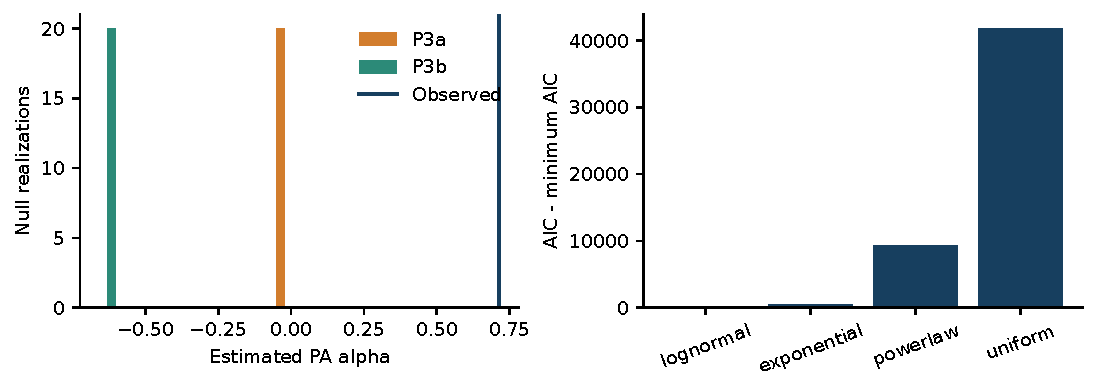
\includegraphics[width=.95\textwidth]{b_null_and_age_models.pdf}
\caption{CIT null-model attachment exponents and age-kernel AIC differences.
Uniform P3a and calibrated age-only P3b each have 20 independent realizations.}
\label{fig:b-null-age}
\end{figure*}

\paragraph{Fit quality does not establish predictability.}
The full-history sample is 500 of 1,019 papers with at least ten citations by age
15; the forecast sample is 500 of 1,220 eligible papers selected only by having
at least five citations in their first five years. Both samples are drawn with a
fixed seed. Median full-history RMSLE is 0.0736 and median scaled-collapse RMSE
0.0220 (90th percentile 0.0453); 10.2\% of full-history fits hit a parameter bound.
\Cref{fig:b-wsb-fits} is an in-sample diagnostic. Held-out scoring in
\cref{tab:b-forecast} and \cref{fig:b-wsb-validation} provides the separate
predictive test. In particular, a collapse obtained using parameters fitted to
the same curve is not independent evidence for universal citation dynamics.

\begin{figure*}[t]
\centering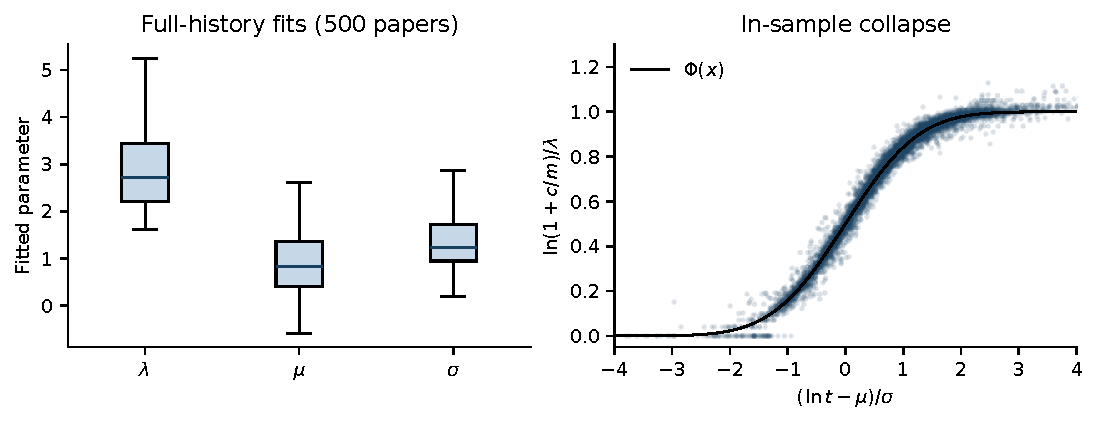
\includegraphics[width=.95\textwidth]{b_wsb_fit_diagnostics.pdf}
\caption{WSB full-history diagnostics: parameter distributions (boxes are
interquartile ranges, median lines, standard 1.5-IQR whiskers; outliers hidden)
and the scaled citation histories against $\Phi(x)$. Parameters are fitted to
ages 1--15, so the collapse is descriptive, not held-out validation.}
\label{fig:b-wsb-fits}
\end{figure*}

\begin{table}[t]
\centering\small
\setlength{\tabcolsep}{4pt}
\begin{tabular}{@{}llrr@{}}
\toprule
Target & Model & MAE & RMSLE\\
\midrule
15 yr & WSB & 15.144 & 0.601\\
 & Linear & 17.064 & 0.662\\
 & No-age PA & 27,588 & 4.601\\
\midrule
2020 & WSB & 28.016 & 0.778\\
 & Linear & 27.271 & 0.876\\
 & No-age PA & $2.79\!\times\!10^6$ & 7.000\\
\bottomrule
\end{tabular}
\caption{Matched forecasts on 500 selected papers using only years 1--5 for
training. The 2020 target is the observed, censored corpus endpoint.
The exponential no-age PA baseline over-extrapolates; beating it alone is a weak
test. The paired MAE intervals against linear both include zero.}
\label{tab:b-forecast}
\end{table}

\paragraph{Sensitivity of the conclusions.}
\Cref{tab:b-robustness} reports time splits, cutoff and corpus-selection checks.
The sign of degree preference and superlinear full-period growth persist, but
$a$ is substantially weaker in the late period. Degree offsets 0.5 and 2 give
$\alpha=0.604$ and 0.858, so the numerical exponent is convention-dependent.
Including 5,486 year ties gives $a=1.324$; ties remain excluded from the primary
DAG. Effective-diameter endpoint estimates remain 6 hops with 64, 128 or 256
sources. First-ten versus all-twenty null means of $\alpha$ are 0.00055/0.00059
(P3a) and $-0.65320$/$-0.65118$ (P3b).
Lognormal ageing is preferred in all target cohorts and both observation halves,
but the recent cohort's fitted tail extends beyond its observed follow-up.
These checks support qualitative stability without eliminating coverage bias,
right censoring or unobserved fitness.

\begin{table}[t]
\centering\small
\begin{tabular}{@{}lrr@{}}
\toprule
Variant & $\alpha$ & $a$\\
\midrule
1990--2020 (primary) & 0.714 & 1.343\\
1990--2004 & 0.684 & 1.455\\
2005--2020 & 0.721 & 1.065\\
Cutoff 2015 & 0.722 & 1.427\\
Core venue families & 0.731 & 1.410\\
Same-year edges included & -- & 1.324\\
\bottomrule
\end{tabular}
\caption{CIT robustness from the saved run. Core venue families contain 14,235
nodes and 47,009 primary edges; the year-tie variant is structural only.}
\label{tab:b-robustness}
\end{table}

\subsection{Measured hypothesis summary}
\label{sec:r-cross}
% Owner: A for eventual cross-network synthesis; B supplies the measured CIT cells.
\Cref{tab:cross} separates available CIT evidence from pending PS/CM experiments.
No ordering of network types by temporal sensitivity is established until the
same normalized measures have been computed for all applicable datasets.
The split H4 verdict avoids treating densification, diameter shrinkage,
descriptive fit and predictive superiority as one interchangeable claim.

\begin{table}[t]
\centering\small
\setlength{\tabcolsep}{4pt}
\begin{tabular}{@{}lcc p{3.8cm}@{}}
\toprule
ID & PS & CM & Measured CIT evidence \\
\midrule
H1 & Pending & Pending & Relative ranges: density/degree 1.798, clustering 2.361, LCC 1.114.\\
H2 & Pending & Pending & --\\
H3 & Pending & Pending & --\\
H4a & -- & -- & $\alpha=0.714$ [0.693, 0.730]; sublinear degree preference.\\
H4b & -- & -- & Lognormal preferred; scale 6.41 yr; $\Delta$AIC versus exponential 537.8.\\
H4c & -- & -- & $a=1.343$; $D_{90}=6$ throughout. Densification, no detected shrinkage.\\
H4d & -- & -- & Compact fits; MAE advantage over linear unresolved.\\
H5 & Pending & Pending & --\\
H6 & Pending & Pending & --\\
H7 & Pending & Pending & --\\
\bottomrule
\end{tabular}
\caption{Available evidence. Pending denotes unmeasured PS and CM experiments;
-- denotes inapplicability. CIT intervals are descriptive year resamples.
H4c/H4d have mixed verdicts. Values come from the shared summary and supporting tables.}
\label{tab:cross}
\end{table}
       % summary  (A assembles)

\FloatBarrier
